\documentclass[a4paper,11pt]{report}
\usepackage[T1]{fontenc}
\usepackage{imakeidx}
\usepackage[pdftex, bookmarks, colorlinks, breaklinks]{hyperref}
\usepackage{graphicx}
%% Code
\usepackage{listings}
\usepackage{xcolor}

\definecolor{codegreen}{rgb}{0,0.6,0}
\definecolor{codegray}{rgb}{0.5,0.5,0.5}
\definecolor{codeorange}{rgb}{1,0.49,0}
\definecolor{back}{rgb}{0.95,0.95,0.96}
%% Dockerfile
\lstdefinestyle{docker}{
    backgroundcolor=\color{back},
    commentstyle=\color{codegray},
    keywordstyle=\color{codeorange},
    nuberstye=\tiny\color{codegray},
    stringstyle=\color{codegreen},
    basicstyle=\ttfamily\footnotesize,
    breakatwhitespace=false,         
    breaklines=true,                 
    captionpos=b,                    
    keepspaces=true,                 
    numbers=left,                    
    numbersep=5pt,                  
    showspaces=false,                
    showstringspaces=false,
    showtabs=false,                  
    tabsize=2,
    xleftmargin=10pt,
}
%% bash

\lstdefinestyle{bash}{
    backgroundcolor=\color{back},
    commentstyle=\color{codegray},
    keywordstyle=\color{codeorange},
    nuberstye=\tiny\color{codegray},
    stringstyle=\color{codegreen},
    basicstyle=\ttfamily\footnotesize,
    breakatwhitespace=false,         
    breaklines=true,                 
    captionpos=b,                    
    keepspaces=true,                 
    numbers=left,                    
    numbersep=5pt,                  
    showspaces=false,                
    showstringspaces=false,
    showtabs=false,                  
    tabsize=2,
    xleftmargin=10pt,
}
%%Python

\lstdefinestyle{python}{
    backgroundcolor=\color{back},
    commentstyle=\color{codegray},
    keywordstyle=\color{codeorange},
    nuberstye=\tiny\color{codegray},
    stringstyle=\color{codegreen},
    basicstyle=\ttfamily\footnotesize,
    breakatwhitespace=false,         
    breaklines=true,                 
    captionpos=b,                    
    keepspaces=true,                 
    numbers=left,                    
    numbersep=5pt,                  
    showspaces=false,                
    showstringspaces=false,
    showtabs=false,                  
    tabsize=2,
    xleftmargin=10pt,
}
%% Define cover
\usepackage{eso-pic}
\usepackage{transparent}

\newcommand\DockerB{%
\put(200,-350){%
\parbox[b][\paperheight]{\paperwidth}{%
\vfill
\centering
{\transparent{0.4} 
\includegraphics[width=15cm,height=15cm,%
keepaspectratio]{img/docker.pdf}}%
\vfill
}}}

\newcommand\OllamaB{
\put(-200,-350){
    \parbox[b][\paperheight]{\paperwidth}{
\vfill
\centering
{\transparent{0.7}
\includegraphics[width=5cm, height=5cm,%
keepaspectratio]{img/ollama.pdf}
}
\vfill
}}}

\newcommand\OldapB{
\put(-230,270){
    \parbox[b][\paperheight]{\paperwidth}{
\vfill
\centering
{\transparent{0.4} 
\includegraphics[width=30cm, height=30cm, keepaspectratio]
    {img/ldap.pdf}
}
\vfill
}}}
\renewcommand{\contentsname}{Index} %index

\begin{document}
% Back images
\AddToShipoutPicture*{\OldapB}
\AddToShipoutPicture*{\DockerB}
\AddToShipoutPicture*{\OllamaB}

\begin{titlepage}
    \begin{center}
        \vspace*{\baselineskip}
        % AUTHOR
        {\Large Gianmiriano Porrazzo}\\
        \vspace*{0.167\textheight}
        % TITLE AND SUBTITLE
        \textbf{\LARGE Cybersecurity-M}\\[\baselineskip] % First title line
	
        {\textcolor{Red}{\Huge Deception Component \\ Generator}}\\[\baselineskip] % Main title line which draws the focus of the reader
	
	      {\Large \textit{LDAP server}} % Subtitle
	
	\vfill % Whitespace between the titles and the publisher
	
    \end{center}
\end{titlepage}

\ClearShipoutPicture

    %%%%%%% INDEX %%%%%%%%%%%%%%
    \tableofcontents
    %%%%%%% INTRODUCTION %%%%%%%
    \chapter*{Introduction}
Defensive deception is one of the methods that cybersecurity experts have started to use. This technique consists in creating fake services and components that appear as valuable targets to attackers.
In that way defenders can divert the attacker’s attention and resources away from critical assets.\\\\
This approach is known as \textbf{Cyber denial and deception} and has as main focus to delay the attack operation, understand the tools and techniques used by the attackers and push the threats into a safe area.\\
By the definition given, deception's goals are two-fold:
\begin{itemize}
    \item provide false or misleading information to the attacker, but capable to give him the belief and confidence that the attack is being performed on real data. This is called \emph{Deception}.
    \item create uncertainty about the reality of the environment that the attacker is facing, to slow down the attacking operations or lead it to waste its time and resources. That is \emph{Denial}.
\end{itemize}
\\\\
Thaks to that attackers spend time and effort trying to compromise these fake elements, leaving less capacity to target the actual valuable asset. 
\\\\
The goal here is to create a deception component for a ldap server. A ldap server could be used to access information about an organization, such as who the employees are and what role they have or also password an personal information if present in the directory. 
\\\\
To reach the goal i used docker to have an easy way to deploy the service and at the same time allow personal configuration and create, update and populate the directory managed by the LDAP protocol. 
\\\\
Now the cybersecurity expert can quickly generate the data, create the docker container, run it and have a distraction for a potential attacker. 
\\\\
In the following i'll describe the whole process in detail.



    %%%%%%% WHAT IS LDAP %%%%%%%
    \chapter{What is LDAP}
Before starting to create the deception component generator, it's usefull to understand what LDAP is.
\\\\
LDAP \cite{ldap} stands for Lightweight Directory Access Protocol, so it’s a protocol to make queries and modify a directory service.  
\\
In fact, the protocol does not include a directory service per se, but some implementations of it also have an integrated one. 
\\
At the beginning, the LDAP protocol was conceived to create an alternative for the DAP protocol, in particular a less resource intensive and lighter one. LDAP was also conceived to use the TCP/IP protocol to make operation related to the X.500 directory easier.  
\\\\
The LDAP protocol has been updated over the years and now it’s at the third version. 
\\
In his version, the simple authentication and security layer (SASL) was added, which is a framework for authentication and security in the internet protocols. 
\section{How it works}
As previously mentioned, the directory could be a generic one, that is possible thanks to the interface, called DataBase Interface easily implementable in a module to guide the beckend. 
\\
The DBI manages a collection of entry or objects. The entries are a composed by attributes, which have a type and one or more values. Every entry has a Distinguish name (DN), that also indicate the position from the root.
\\
The entries are also hierarchically ordered, and the final structure is called DIT (Directory Information Tree) and is a way to store the representation of the DB managed by the DBI.
\begin{figure}[h]
    \caption{How LDAP works}
    \centering
    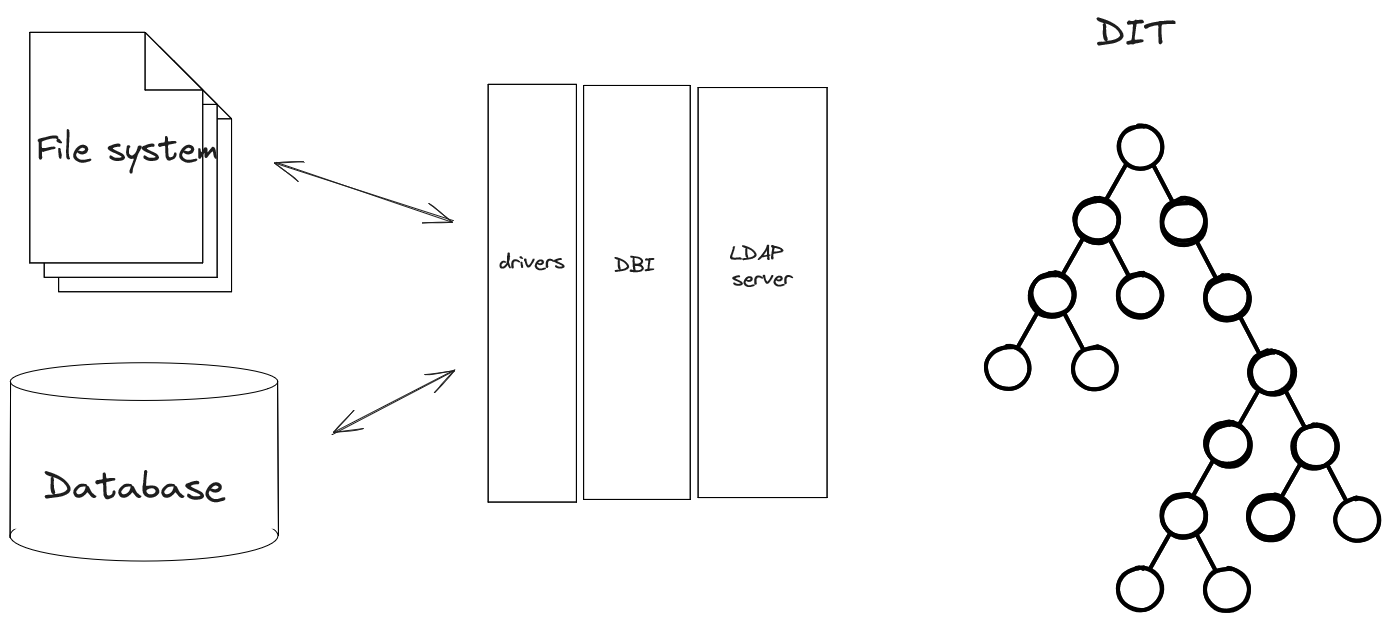
\includegraphics[width=15cm]{img/arch.png}
\end{figure}
\\
It is used a hierarchy because LDAP was born as a system to organize data about people and resources inside a company. The hierarchy also allows us to make direct links to the data, an easy partitioning system to administrate, control the access and locate easily data. 
\\\\
An entry is a collection of the attributes, in which the value of it is stored directly, and it’s labeled by the type of itself.
\\
Between the various possible attributes, two must be indicated: dn and one or mode objectClass. This format is also used to exchange entries between client and server, and is called LDIF (LDAP interchange format). 
\\
For inserting an entry it’s necessary to have well formatted objects and a uniform view of the data, commonly used between all the users. This is the function of a SCHEMA. A schema is a set of rules that describes the data and have two types of definitions: 
\begin{itemize}
    \item ObjectClass 
    \item attributeType 
\end{itemize}
\\
Every entry is based on one or more objectClass, which describes the types of attributes that must or should be in the entry.  Every attribute has its own type, with also the set of rules necessary to compare them. 
\\
The attribute type can be one of the commonly used or can also be described by the user, but in that case, it must be defined in a file and added to the server configuration. It can be done using the ldif format or a schema file.
\\
This is valid also for objectClass.
\begin{mdframed}[backgroundcolor=back1]
    \begin{lstlisting}[style=bash, caption={Example of definition of an attributeType (for objectClasses is similar)}]
olcAttributeTypes: (...)
    DESC 'name'
    EQUALITY caseMatch
    SUBSTR caseMatchSubs
    SYNTAX ....
    \end{lstlisting}
\end{mdframed}
\begin{figure}[h]
    \caption{Correspondance between schema definition and DIT elements}
    \centering
    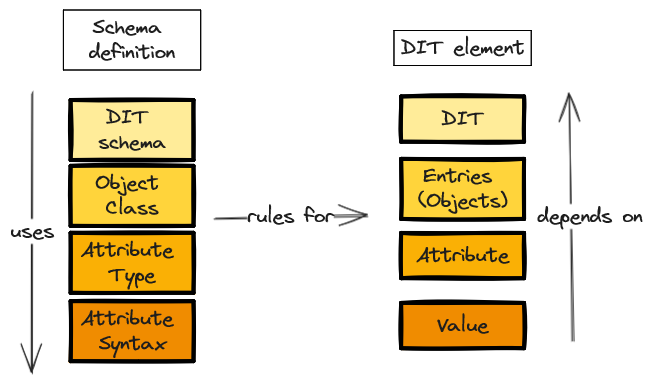
\includegraphics[width=15cm]{img/dit.png}
\end{figure}
\\\\
One famous implementation of LDAP is OpenLDAP \cite{openldap}, which includes the Access protocol and a directory. This is the one choosen to create the docker image to configure.
%% TODO: insert OpenLdap logo

    %%%%%%% WHAT IS DOCKER %%%%%
    \chapter{Docker}
Docker \cite{docker} is a set of PaaS products that uses OS virtualization to deliver software in packeges called containers. A container is a unit of software that packages up software and its dependencies, so the application runs and could also be shared. 
\\\\
To develop a docker container there are several options: one is to create a Docekerfile in which we can detail all the specifications and the features that we want to run in that container. Usually that is to run a single application in a sandbox environment.  
\\
In the study case the application is an OpenLDAP server. To run that it’s needed an operating system: the choice i made is to use a debian image.
\section{Creation of the container}
\begin{mdframed}[backgroundcolor=back]
\lstinputlisting[style=docker]{code/Dockerfile}
\end{mdframed}
Once the base image is chosen, it is necessary to install the package that will be used. The list of packages is shown in the figure. In particular slapd is the daemon that runs the ldap server, ldap-utils contains all the tools to search, add, modify and delete entries from the server from the outside. The others contains usefull tools that will be used in the next steps.  
\\
After that it is made a copy of the deception and configuration data inside the conteiner, and are exposed two ports for reach the container from the outside. Two ports because one is for the base TCP connection (10389) and one for the connection using TLS (10636). 
\\
At the end of the Dockerfile it’s launched a script that configures the server.
\section{Configuration scripts}
The script is writen in bash and call starts and configure a daemon used in the data generation and calls two other scripts:
\begin{itemize}
    \item the first is used to reconfigure the server
    \item the second is used to run the server using the specified ports
\end{itemize}
\\
In the first scripts are present four functions:\\
\begin{itemize}
    \item \textit{reconfigure\_slapd()}
    \item \textit{configure\_admin\_conig\_pw()}
    \item \textit{load\_initial\_data()}
    \item \textit{convert\_schema()}
\end{itemize}
\\
The first one configures the server using the info submitted in the Dockerfile. This step is needed because when slapd is installed it creates a default config, so to modify the dafault paramenters we use that function.
\\
The \textit{configure\_admin\_config\_pw()} insert the info of a specific ldif file that contains data about the adimn.
\\
\textit{load\_initial\_data()} finds all the ldif files inserted into the copied folder and add them following a specified order (in our case the order is taken from the file names).
\\
The last function converts the .schema files into .ldif definitions, using the tool \textbf{schema2ldif} \cite{schema2ldif} and add them into the directory.
\\
After that configuration steps the server is created. To allow it to run on the exposed ports, it's stopped and reactivated using the following script.
\begin{mdframed}[backgroundcolor=back]
\lstinputlisting[style=bash]{code/slapd-init.sh}
\end{mdframed}
Once generated the Dockerfile and the relative configuration we can run the container and see that it works.
\begin{figure}[h]
    \caption{Example of working container}
    \centering
    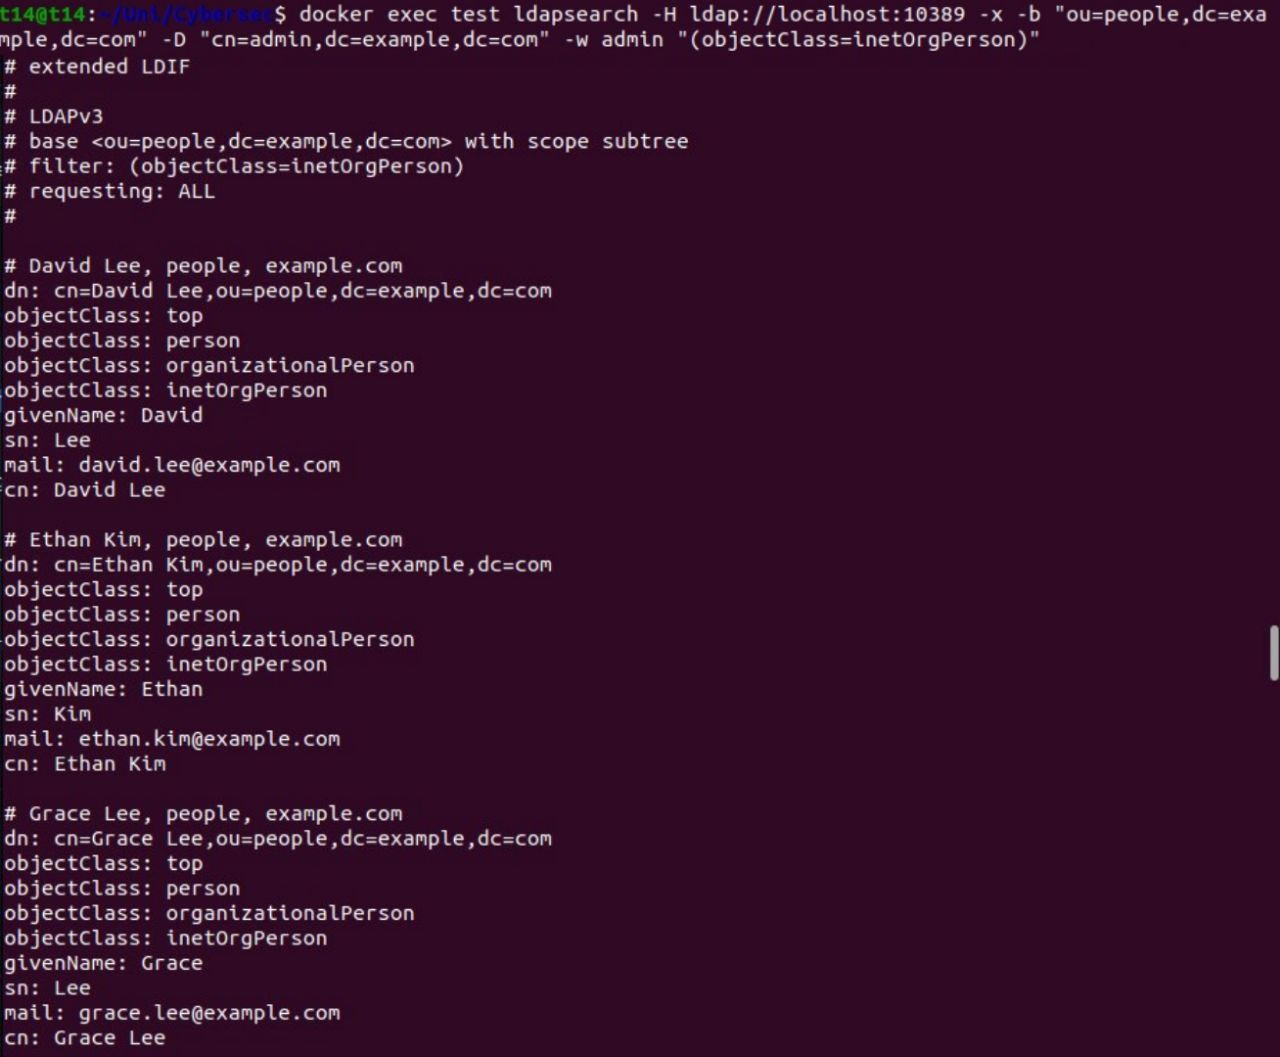
\includegraphics[width=10cm]{img/search.jpg}
\end{figure}

    %%%%%%% DATA GENERATION %%%%
    \chapter{Data generation}
To make the deception component generator a real one, it's necessary to have some data to insert into it.
For generate this datas i've used one of the most talked technologies of our time: Large Language Models. In fact this is a task that they do well.
\\
As first step i've had to decide which LLM use: the model choosen is LLAMA2, principally because it's an open source project and it is possible to run it locally.
Done that i've used langchain \cite{langchain} to write a simple python script that generates the data. But before that it was necessary to find a way for use a LLM locally.
\section{Problem}
The benefit of running it locally have a cost: the precision of the model depends on the machine in which it's running. Eveni if the model is pretrained, depending on some parameters, the model could run better or worse.
\\\\
To fix this problem i had to choose in which way run the model. So two were the possible approaches:
\begin{itemize}
    \item use llama-cpp-python package
    \item use ollama
\end{itemize}
\section{llama-cpp-python}
This is a project born to create an interface to use llama-cpp in python \cite{llama-cpp-python}.
After setting up the environment, and create a python script to generate data (even inside the docker itself), what we can see is that the data generated are not so heterogeneous and it needs a lot of time to generate them.
%% TODO: image
Another negative aspect is that i've to download the model and insert it in the docker to make it run, so the docker grows in its weight.
\section{ollama}
To avoid all this problems i have decided to use Ollama \cite{ollama}. Ollama is a recent created project thatmakes users run LLMs locally in a docker-like way. So even in this case you have to download your model, but now we do not need to insert in our docker file.
\\
The idea is to generate data before, save it and then upload them in the docker.
Here we can see a more heterogeneous data creation. Even if there are changes to be made to make it works, it's bettere than the previous output.
%% TODO: insert image
After finding ollama, i've started to think on how i could implement it in a python script to make it generate random data when the docker is started.
\\
After reading the documentation online i've found a way to do so:
\begin{mdframed}[backgroundcolor=bpy]
\lstinputlisting[style=python]{../../init/ollama.py}
\end{mdframed}

\\
Analyzing that i've observed that it needs some time to run, but at least it creates a valid number of random data. 
\\\\
So now i've created the docker for the service, with the possibility to configure it and generate deception data: the last think to do is try to deploy it.

    %%%%%%% DEPLOY %%%%%%%%%%%%%
    \chapter{Deploy}
Once understood how create the server and generate the data to insert into it, the last phase is deploy the product.
\\ 
Before that what i've had to do is create a OCI image, from the Dockerfile, using the docker build, command.
\\
After that i can run the OCI image, as follow:
%% TODO: oci image
Now everithing is ready and setted up, so a cybersecurity expert can download the image and run it with randomly generated data, that use a Ollama to generate them.

    %%%%%%% END %%%%%%%%%%%%%%%%
    \chapter{Final considerations}
The creation of a deception component was possible going through different phases.
\\
At the beginning i've had to understand the service that was chosen to be duplicated with random data, after i've had to understand how create a Dockerfile to create it and make configuration possible and, at the end, the main point of all is how to generate credible data to insert into it.
\\\\
This was the main task, because some LLM runned locally performed not so good for what i was aimning to do. So to solve that i gave a quick look at the possibility to define a grammar in llama-cpp-python, to get a precise output. Unfortunately even doing so the generated data were not so credible and structured, so it was difficult to have an ldif as the final output.
\\
After some research i've found the Ollama project and i've tried to use it for that purpose. Even if in that case there's no possibility for use a specific grammar for the output, i've obtained a more credible output and in a more ldif compatiple syntax. This is also because it's possible to insert a template to generate an output that looks alike it: in that way i have a more precise output and i can use it to produce a file that follow the ldif syntax.
\\\\
At the end of all i've created the OCI image for the LDAP server with all the needed features.
\\\\
One consideration that i can made about this is that using LLM in a docker make it grow in size a lot, because it has to have the model installed to run it and generate the data. All that can make the installation slower and the container pretty heavy. One solution that could be applied is to have a different machine or a different container, that act like a server, in which run the choosen model and make requests to it to make it generate data. In that way we could have lighter and faster containers.
\\\\
Except for this detail, now the container is finished and everyone can, using some commands, create a fake LDAP server with data in it generated automatically. So we can divert an attacker to target that service instead a real one and make it to loose time and resources doing that.

\end{document}
